\chapter{دورة المسح من البداية إلى النهاية}
\label{ch:quick-cycle}
\section{الدورة في مخطط واحد}
\label{sec:quick-map}

يمر كل مسح بست مراحل ثابتة. تُدخل المنشآت وتجهّز فرق البحث، ثم تهيّئ النماذج والاستبيانات، ثم تعمل خطة بتكليفات. بعدها يجري الباحثون المسح، ويتحقق المراجعون من البيانات، وتراقب الإدارة لوحات المؤشرات. كل مرحلة تبني على نتيجة التي قبلها، فلا تبدأ مرحلة قبل أن تكتمل سابقتها.

\begin{figure}[H]
\centering
\begin{tikzpicture}[node distance=0.4cm,stepBox/.append style={minimum width=8.4cm,text width=8cm,minimum height=0.7cm}]
  \node[stepBox] (s1) {\RL{المنشآت وفرق البحث}\\\RL{ملف المنشأة · الباحث}};
  \node[stepBox,below=of s1] (s2) {\RL{النماذج والاستبيانات}\\\RL{قواعد · مراجعة · حزمة}};
  \node[stepBox,below=of s2] (s3) {\RL{خطة التكليفات}\\\RL{منشآت · موعد · جولة}};
  \node[stepBox,below=of s3] (s4) {\RL{عمليات المسح}\\\RL{تعبئة · تحقق · إرسال}};
  \node[stepBox,below=of s4] (s5) {\RL{التحقق من البيانات}\\\RL{تقييم · تصحيح · توقيع}};
  \node[stepBox,below=of s5] (s6) {\RL{لوحات المؤشرات}\\\RL{تقدم · لوحة · إغلاق}};
  \draw[flowsTo] (s1) -- (s2);
  \draw[flowsTo] (s2) -- (s3);
  \draw[flowsTo] (s3) -- (s4);
  \draw[flowsTo] (s4) -- (s5);
  \draw[flowsTo] (s5) -- (s6);
\end{tikzpicture}
\caption{مراحل دورة المسح الست}
\label{fig:quick-flow}
\shotnote{يبيّن المخطط ترتيب العمل، وتحت اسم كل مرحلة أهم ما تشمله. المهم فيه أن كل مرحلة تحتاج إلى نتيجة سابقتها: فلا خطة بلا حزمة منشورة، ولا مراجعة بلا إرسال. وإذا أُعيدت إجابة للتصحيح في المرحلة الخامسة، رجعت إلى الباحث في المرحلة الرابعة ثم عادت إلى المراجعة.}
\end{figure}

\begin{figure}[H]
\centering
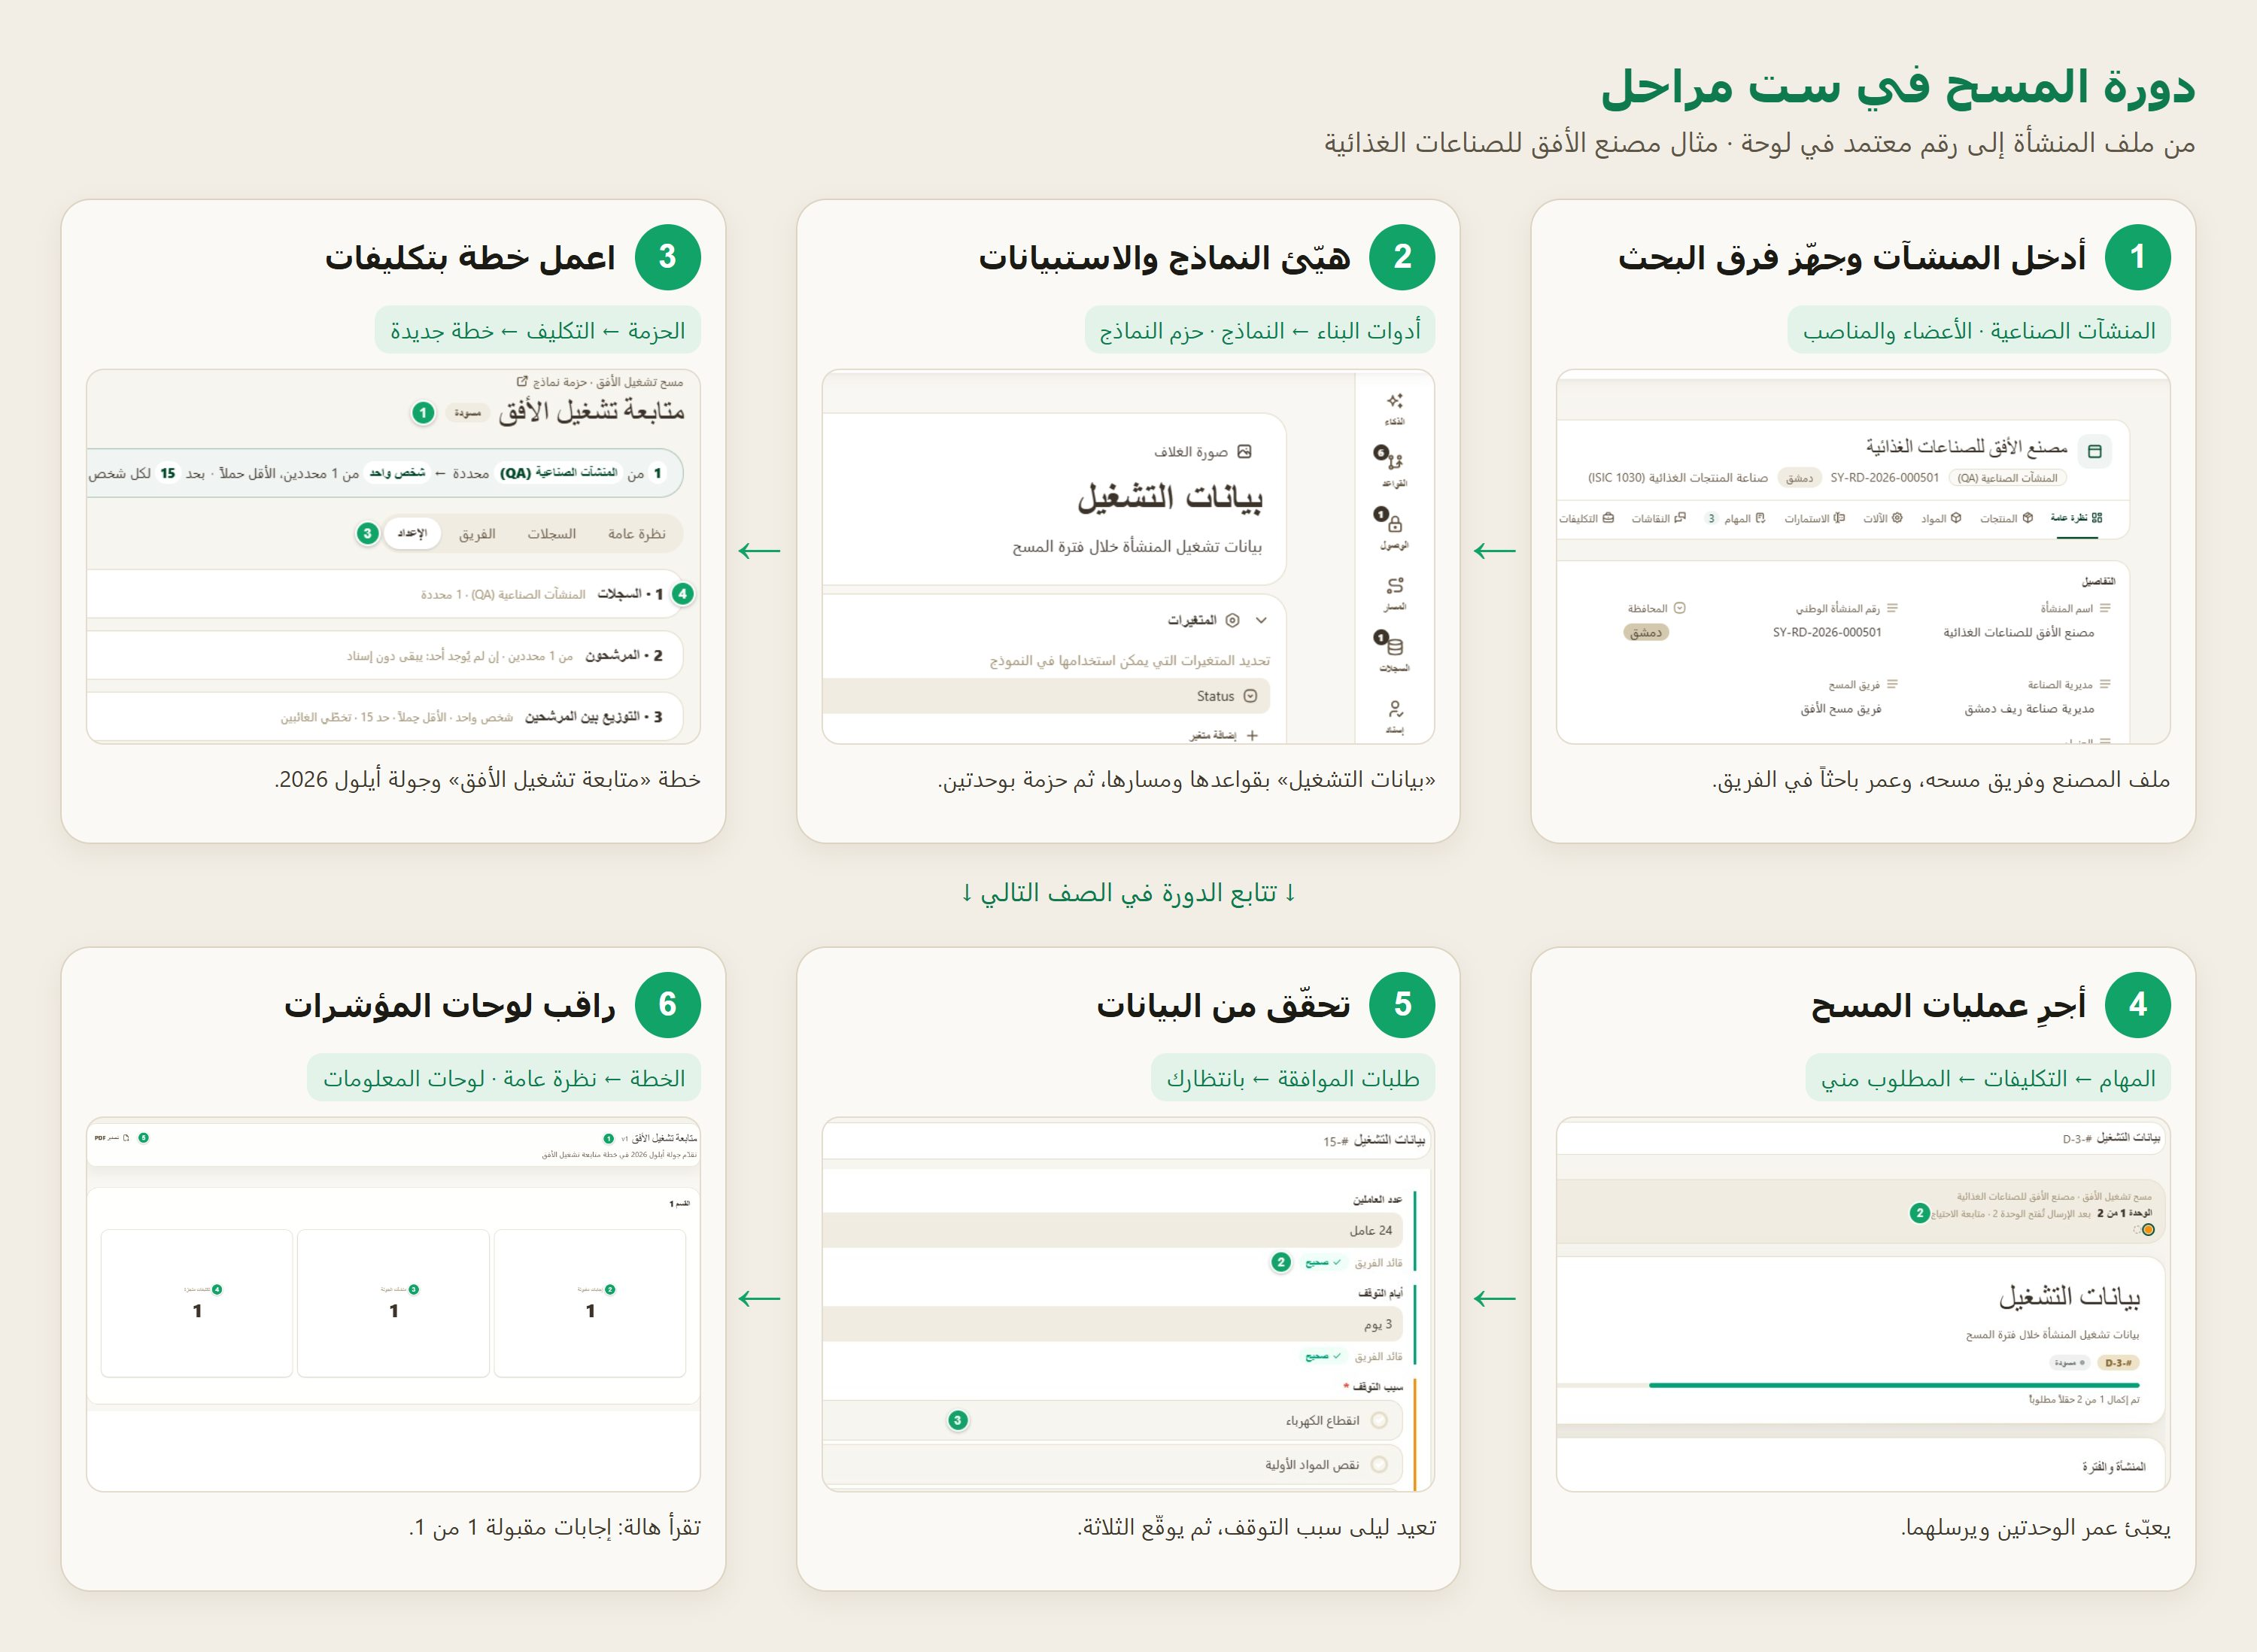
\includegraphics[width=\linewidth]{assets/screens/quick-cycle-ar.jpg}
\caption{المراحل الست كما تظهر في النظام}
\label{fig:quick-chart}
\shotnote{تعرض اللوحة شاشة حقيقية لكل مرحلة، وفوقها مكانها في النظام. تفيدك في التعرف على الشاشة عندما تصل إليها، حتى لو لم تقرأ الفصل كاملاً. وتتبع الأسهم ترتيب المراحل من 1 إلى 6. ① ملف المنشأة. ② منشئ النماذج. ③ إعداد الخطة. ④ التعبئة. ⑤ المراجعة. ⑥ لوحة المؤشرات.}
\end{figure}

\begin{table}[H]
\centering
\caption{أماكن العمل داخل النظام}
\label{tab:quick-places}
\begin{tabularx}{\linewidth}{R{3.4cm} R{2cm} Y R{2.2cm}}
\rcHeaderRow
\thh{المرحلة} & \thh{من؟} & \thh{أين في النظام؟} & \thh{التفاصيل}\\
1. المنشآت والفرق & يوسف والمسؤول & «المنشآت الصناعية»، والأعضاء والمناصب. & الفصلان~\ref{ch:02-roles} و~\ref{ch:03-register}\\
2. النماذج & سارة & «أدوات البناء» ثم «النماذج»، ثم «حزمة نماذج جديدة». & الفصل~\ref{ch:04-forms}\\
3. الخطة & سارة & الحزمة ثم «التكليف» ثم «خطة جديدة». & الفصل~\ref{ch:05-plans}\\
4. المسح & عمر & «المهام» ثم «التكليفات» ثم «المطلوب مني». & الفصل~\ref{ch:06-assignments}\\
5. التحقق & ليلى وخالد ورنا & «طلبات الموافقة» ثم «بانتظارك». & الفصل~\ref{ch:07-review}\\
6. المتابعة & سارة وهالة & الخطة ثم «نظرة عامة»، و«لوحات المعلومات». & الفصل~\ref{ch:08-results}\\
\end{tabularx}
\end{table}

\begin{rcnote}[المثال في هذه الصفحة]
نتابع منشأة واحدة: «مصنع الأفق للصناعات الغذائية» في ريف دمشق، وجولة واحدة: «أيلول 2026». سارة تعدّ المسح، وعمر يجمع البيانات، وليلى وخالد ورنا يراجعون، وهالة تقرأ النتيجة.
\end{rcnote}

\section{أدخل المنشآت وجهّز فرق البحث}
\label{sec:quick-register}

\textbf{لماذا؟} لا يُكلَّف إلا ما له ملف. فملف المنشأة هو ما تختاره الخطة، وما تقرؤه النماذج، وما تُكتب فيه النتيجة. وفريق المسح في الملف هو ما تعرف منه الخطة باحث المنشأة.

\begin{enumerate}
\item افتح «المنشآت الصناعية»، وأنشئ ملف المنشأة أو تحقق منه: الاسم، والرقم الوطني، والمحافظة، والنشاط، و«حالة التشغيل».
\item اختر في «فريق المسح» الوحدة المسؤولة عن المنشأة.
\item تأكد أن للباحث تعييناً نشطاً في منصب «باحث ميداني» داخل هذا الفريق.
\end{enumerate}

\begin{figure}[H]
\centering
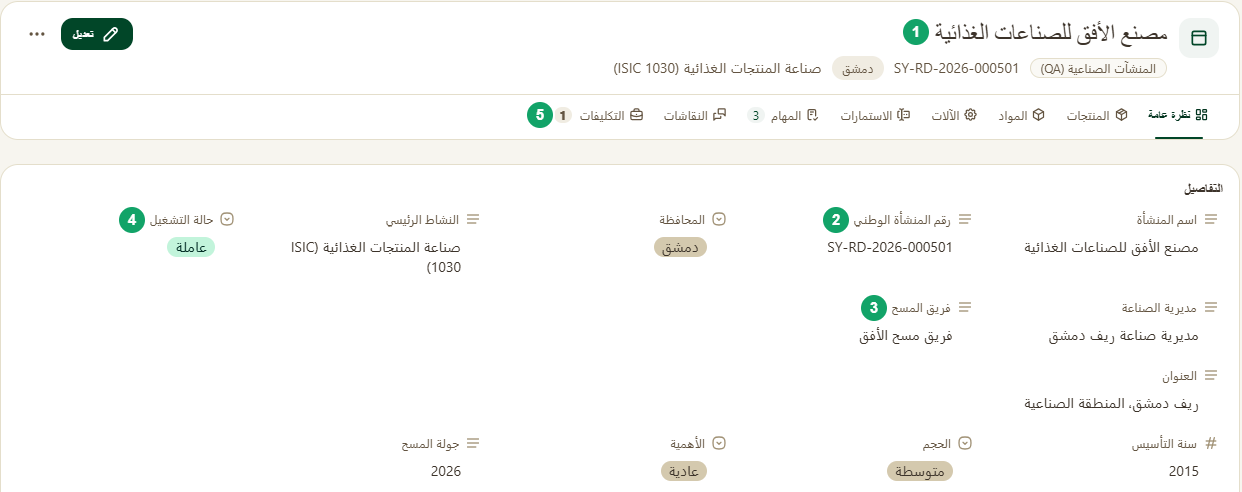
\includegraphics[width=\linewidth]{assets/screens/quick-facility-ar.png}
\caption{ملف مصنع الأفق}
\label{fig:quick-facility}
\shotnote{هذا ملف المنشأة الذي تبدأ منه الدورة كلها. تفيدك قراءته في التأكد من أن المنشأة جاهزة للتكليف قبل بناء الخطة. وتظهر «دمشق» لأنها المحافظة المختارة في بيئة التجربة. ① اسم المنشأة. ② «رقم المنشأة الوطني». ③ «فريق المسح»: منه تأتي الخطة بالباحث. ④ «حالة التشغيل»: «عاملة». ⑤ «التكليفات»: تكليفات المنشأة الحالية والسابقة.}
\end{figure}

\begin{rcnote}[تطبيق المثال]
يتحقق يوسف من ملف مصنع الأفق: «عاملة»، و«فريق المسح» = فريق مسح الأفق. ويعيّن المسؤول عمر في منصب «باحث ميداني - RES» داخل الفريق.
\end{rcnote}

\section{هيّئ النماذج والاستبيانات}
\label{sec:quick-forms}

\textbf{لماذا؟} النموذج يحدد ما يُسأل، وقواعده تمنع الخطأ قبل الإرسال، ومساره يحدد من يراجع. والحزمة تجمع نماذج المنشأة في عمل واحد بترتيب ثابت.

\begin{enumerate}
\item من «أدوات البناء» ثم «النماذج» أنشئ النموذج، وضع أسئلة كل صفحة داخل قسم.
\item أضف سؤال «المنشأة» وفعّل فيه «سؤال سجل»، ثم أضف القواعد من «القواعد».
\item من «المسار» فعّل المسار، وأضف «خطوة موافقة» بمراحل المراجعين، ثم «نشر».
\item أنشئ «حزمة نماذج جديدة»، وأضف النماذج وحدات، وفعّل «سجل الجولة»، ثم «نشر».
\end{enumerate}

\begin{figure}[H]
\centering
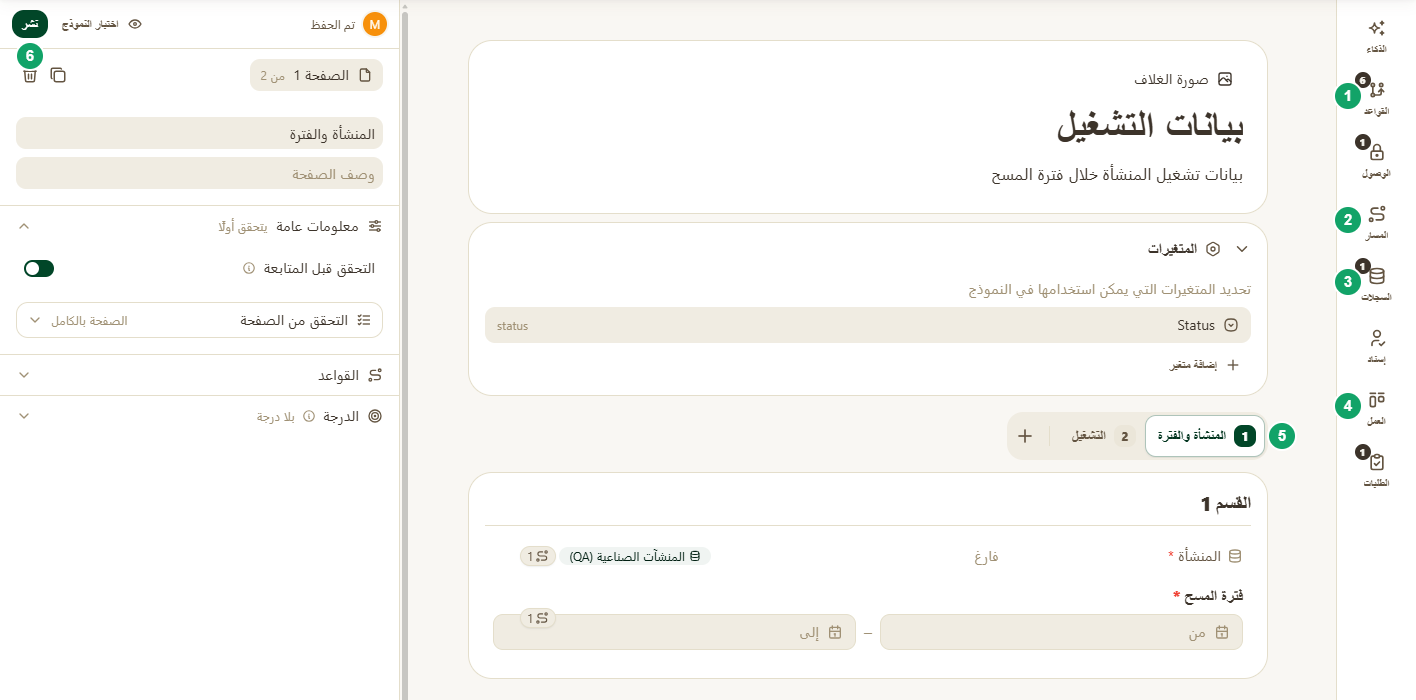
\includegraphics[width=\linewidth]{assets/screens/quick-builder-ar.png}
\caption{نموذج «بيانات التشغيل» في المنشئ}
\label{fig:quick-builder}
\shotnote{هذه شاشة بناء النموذج، وأدواته في الشريط الجانبي. تفيدك في معرفة مكان كل إعداد تحتاجه في هذه المرحلة. والرقم الصغير فوق الأداة عدد ما ضُبط فيها. ① «القواعد». ② «المسار»: المراجعة والتوقيع. ③ «السجلات»: ما يُكتب في الملف بعد الاعتماد. ④ «العمل»: الحزمة والخطة. ⑤ صفحات النموذج. ⑥ «نشر».}
\end{figure}

\begin{rcnote}[تطبيق المثال]
تبني سارة «بيانات التشغيل»: المنشأة، وفترة المسح، وعدد العاملين، وأيام التوقف (0–30)، وسبب التوقف الذي يظهر ويُطلب عند أيام توقف أكبر من 0. مسارها: تدقيق آلي، ثم ليلى، ثم خالد، ثم رنا. ثم تجمعها مع «متابعة الاحتياج» في حزمة «مسح تشغيل الأفق».
\end{rcnote}

\section{اعمل خطة بتكليفات}
\label{sec:quick-plan}

\textbf{لماذا؟} الخطة تحوّل الحزمة إلى عمل موزع: تكليف واحد لكل منشأة، لشخص مناسب، بموعد واضح. فلا تحتاج إلى تكليف المنشآت واحدة واحدة.

\begin{enumerate}
\item افتح الحزمة، ثم «التكليف» ثم «خطة جديدة».
\item اضبط الأقسام الستة: المنشآت، والمرشحين، والتوزيع، والموعد، والمتابعة، ومن يدير الخطة.
\item اضغط «تشغيل المعاينة»، وتأكد أن «دون مرشح» = 0.
\item اضغط «إنشاء التكليفات»، واكتب اسم الجولة وفترتها.
\end{enumerate}

\begin{figure}[H]
\centering
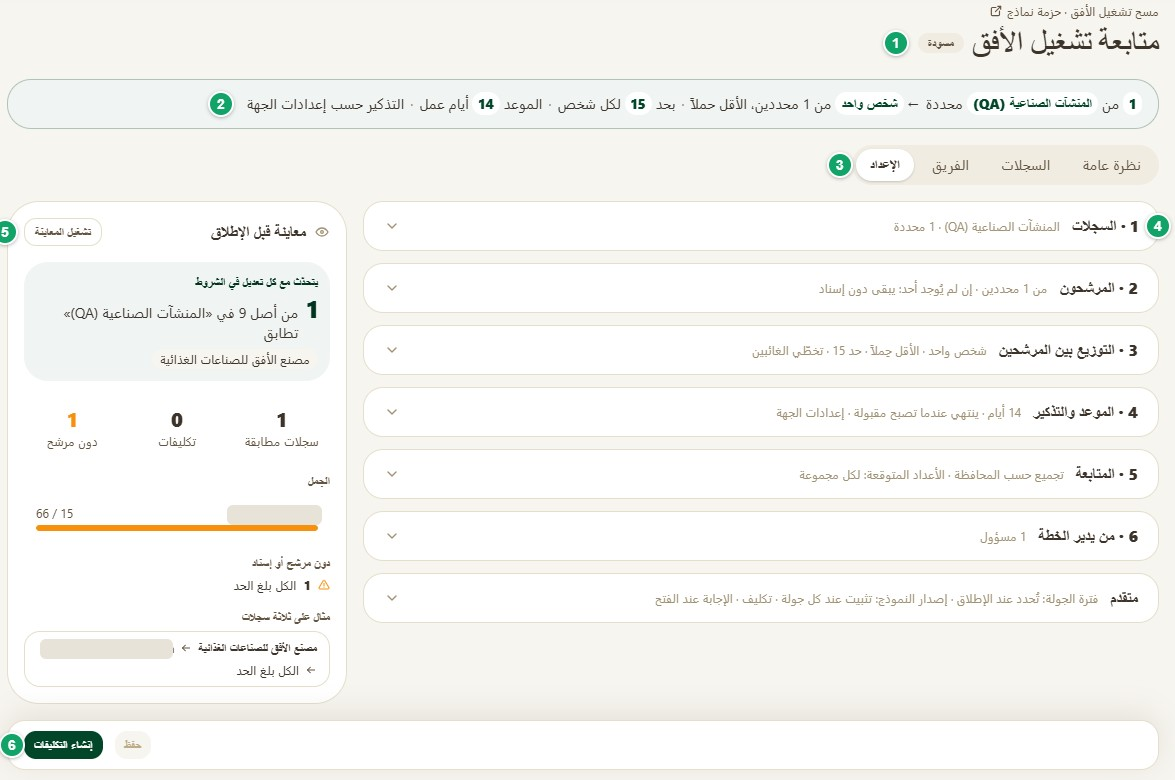
\includegraphics[width=\linewidth]{assets/screens/plans-setup-ar.jpg}
\caption{إعداد خطة «متابعة تشغيل الأفق»}
\label{fig:quick-plan}
\shotnote{هذه صفحة إعداد الخطة، وكل قسم فيها مطوي على ملخص اختيارك. تفيدك المعاينة في الجانب في كشف المنشأة التي لن تُكلَّف قبل الإطلاق. ① الاسم والحالة. ② ملخص الخطة. ③ «الإعداد». ④ الأقسام. ⑤ «معاينة قبل الإطلاق». ⑥ «إنشاء التكليفات».}
\end{figure}

\begin{rcnote}[تطبيق المثال]
تختار سارة مصنع الأفق، والمرشحين من «فريق المسح»، وشخصاً واحداً «الأقل حِملاً» بحد 15، وموعداً 14 يوم عمل ينتهي عند «مقبولة». وتطلق جولة «أيلول 2026»، فيصل التكليف إلى عمر.
\end{rcnote}

\section{أجرِ عمليات المسح}
\label{sec:quick-survey}

\textbf{لماذا؟} هنا تُجمع البيانات من مصدرها. والنموذج يتحقق من كل إجابة لحظة كتابتها، فيصل إلى المراجع ما يستوفي القواعد فقط.

\begin{enumerate}
\item افتح «المهام» ثم «التكليفات» ثم «المطلوب مني»، واضغط «ابدأ الوحدة 1».
\item املأ الأسئلة، وصحّح أي حقل أحمر. يُحفظ كل تغيير تلقائياً.
\item اضغط «إرسال الوحدة» ثم «إرسال الطلب»، ثم أكمل الوحدة التالية من صفحة الحزمة.
\end{enumerate}

\begin{figure}[H]
\centering
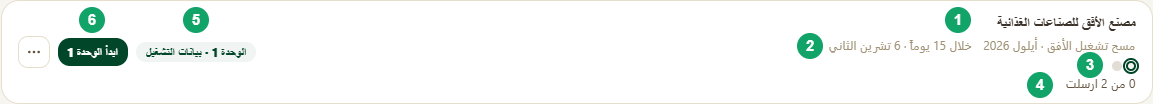
\includegraphics[width=\linewidth]{assets/screens/assignments-card-ar.png}
\caption{بطاقة مصنع الأفق في «المطلوب مني»}
\label{fig:quick-card}
\shotnote{هذه البطاقة نقطة دخول الباحث إلى المسح. تفيده في معرفة المنشأة والموعد والوحدة التالية دون أن يفتح شيئاً. ① اسم المنشأة. ② الحزمة والجولة، ثم الموعد. ③ نقطة لكل وحدة. ④ «0 من 2 أُرسلت». ⑤ الوحدة التالية. ⑥ «ابدأ الوحدة 1».}
\end{figure}

\begin{rcnote}[تطبيق المثال]
يكتب عمر 24 عاملاً، ثم 40 يوم توقف خطأً، فتظهر «أدخل 30 أو أقل.». يصححها إلى 3، ويختار السبب «أخرى»، ويرسل. ثم يرسل «متابعة الاحتياج».
\end{rcnote}

\section{تحقّق من البيانات}
\label{sec:quick-review}

\textbf{لماذا؟} الإرسال لا يعني الصحة. يقيّم المراجعون كل إجابة، ويعيدون الخطأ إلى الباحث بملاحظة على السؤال نفسه، ولا تُقبل الإجابة إلا بعد آخر توقيع.

\begin{enumerate}
\item افتح «طلبات الموافقة» ثم «بانتظارك»، ثم الطلب.
\item قيّم كل إجابة: «صحيح» أو «يحتاج تصحيحًا» مع ملاحظة، أو «لا ينطبق».
\item اختر «موافقة» أو «إعادة للتصحيح» أو «رفض»، ثم وقّع بملف مفتاحك ورمز PIN.
\end{enumerate}

\begin{figure}[H]
\centering
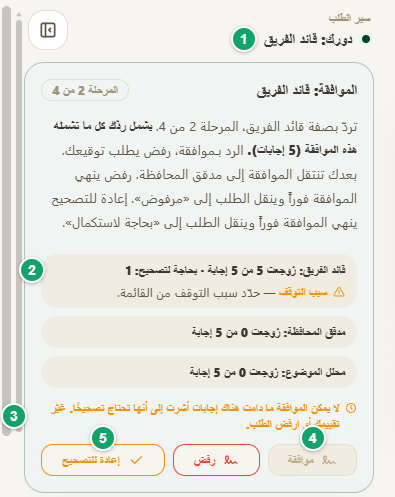
\includegraphics[width=0.62\linewidth]{assets/screens/review-decision-ar.png}
\caption{لوحة القرار عند قائد الفريق}
\label{fig:quick-review}
\shotnote{تعرض اللوحة دور المراجع، وما قيّمه، والقرارات المتاحة له. تفيده في معرفة سبب تعطل الموافقة قبل أن يقرر. ① «دورك: قائد الفريق». ② ملخص التقييم والسؤال المؤشَّر عليه. ③ سبب تعطل الموافقة. ④ «موافقة». ⑤ «إعادة للتصحيح».}
\end{figure}

\begin{rcnote}[تطبيق المثال]
يقترح التدقيق الآلي أن «أخرى» تحتاج تصحيحاً. توافقه ليلى وتعيد الإجابة بملاحظة «حدّد سبب التوقف من القائمة.». يختار عمر «انقطاع الكهرباء» ويرسل، فتوقّع ليلى ثم خالد ثم رنا، وتصبح الإجابة «مقبول».
\end{rcnote}

\section{راقب لوحات المؤشرات}
\label{sec:quick-monitor}

\textbf{لماذا؟} الأرقام المقبولة هي التي تُبنى عليها القرارات. تتابع سارة التقدم في الخطة، وتقرأ هالة الصورة العامة في لوحة، ثم تُغلق الجولة لتثبت بياناتها.

\begin{enumerate}
\item افتح الخطة ثم «نظرة عامة»: «معتمدة» و«متأخرة» و«حسب المحافظة».
\item أنشئ لوحة من «لوحات المعلومات»، وعنصراً مصدره «خطة تكليف»، ثم «نشر».
\item عند انتهاء الفترة اختر «إغلاق الجولة»، ثم «تشغيل جولة جديدة» للفترة التالية.
\end{enumerate}

\begin{figure}[H]
\centering
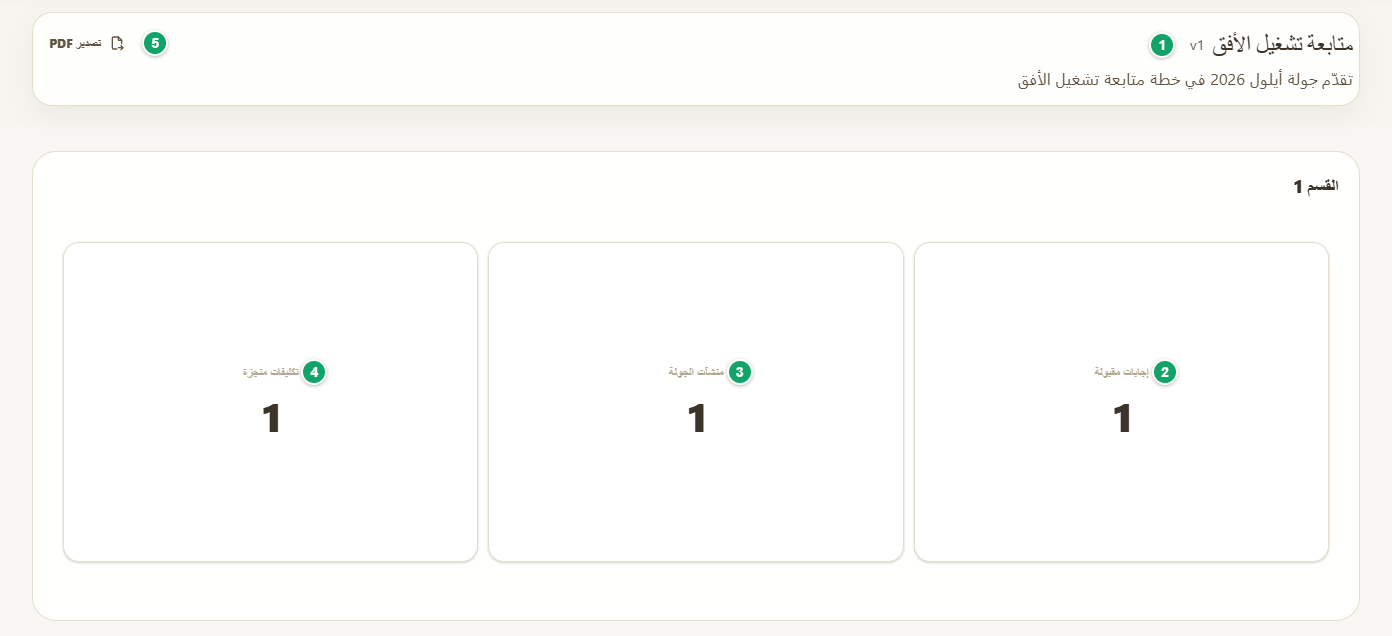
\includegraphics[width=\linewidth]{assets/screens/results-dash-view-ar.png}
\caption{لوحة «متابعة تشغيل الأفق»}
\label{fig:quick-dashboard}
\shotnote{هذه اللوحة كما تقرؤها الإدارة، وأرقامها تأتي من الخطة مباشرة. تفيد في متابعة المسح دون فتح الخطة أو تفاصيل المنشآت. ① اسم اللوحة. ② «إجابات مقبولة». ③ «منشآت الجولة». ④ «تكليفات منجزة». ⑤ «تصدير PDF».}
\end{figure}

\begin{rcnote}[تطبيق المثال]
تجد سارة «معتمدة 1» و«متأخرة 0»، وريف دمشق بلغ عدده المتوقع. وتقرأ هالة في اللوحة: إجابات مقبولة 1، ومنشآت الجولة 1، وتكليفات منجزة 1. وفي نهاية أيلول تغلق سارة الجولة.
\end{rcnote}

\begin{rcchecklist}[الدورة مكتملة عندما]
\begin{checklist}
\item للمنشأة ملف وفريق مسح، وللفريق باحث معيّن.
\item النموذج والحزمة منشوران، ومسار المراجعة مضبوط.
\item الخطة نشطة، وكل منشأة لها تكليف.
\item أُرسلت الوحدات كلها.
\item وقّع كل المراجعين، وصارت الإجابات «مقبولة».
\item تعرض الخطة واللوحة الأرقام نفسها، وأُغلقت الجولة بعد انتهاء فترتها.
\end{checklist}
\end{rcchecklist}
